\section{Calculation of the branching fraction}

The signal yield of the decay \btodsphi is determined by performing an unbinned maximum likelihood
fit to the invariant mass spectrum of the candidate \Bp mesons.
The fit is done simltaneously to the four regions indicated in \Tab{tab:dsphi:hel}, this enables
additional constraints to be placed on the background distribution.
In the fit, there are several components: the signal \btodsphi; combinatorial background; and
specific backgrounds that peak below the \Bp mass.

The signal shape is a Gaussian function with parameters that were fixed from a fit to simulated
events.
It is also determined from simulation that the total signal is distributed between the regions:
\rA 89\pc, \rB 4\pc, \rC 7\pc, and in \rD there is no signal expected.
Therefore, the region \rA is the signal region, and \rD is solely background.
These additional fit regions allow the background components to be determined very precicesly.

The $\phi$ from the decay \btodsstrphi does not need to be longitudinally polarized because the
\Dssp is a vector meson ($J^P=1^-$), and therefore the value of $\cos\thetahel$ is uniformly
distributed between zero and one.
The photon from the decaying \Dssp is not reconstructed, and therefore the background from the
decay \btodsstrphi peaks below the nominal \Bp mass.

Other sources of background that peak below the mass of the \Bp meson are from the decay modes
$\decay{\Bsb}{D_s^{(*)+}\Kstarz\Km}$.
These arise when the pion from the \decay{\Kstarz}{\Kp\pim} is not reconstructed.
Since there is missing energy from the pion (and photon in the case of the \Dssp decay), these peak
significantly below the \Bp mass.
However, their background shapes are non-trivial, and a good understanding of them is vital in
understanding the background component that is directly under the signal component.

The background shapes for \btodsstrphi and \bstodskstrk are taken from simulated events,
reconstructed as \btodsphi candidates.
Since the shapes of these reconstruced candidates are non-trivial, a kernel density estimation
technique~\cite{Cranmer:2000du} is used to understand these shapes.

There were no simulated events available with which to understand the shape of the \bstodsstrkstrk
background.
Instead the shape taken from the \bstodskstrk background is convolved with a distribution
parameterising the loss of a photon (or pion) as seen between the decays \btodsstrphi and
\bstodskstrk.

The shapes of peaking background contributions are taken from kernel density
estimates of simulated events, as described.
Yields of background components are also fixed from...
Therefore, the only floating parameters in the simultaneous fit is the total signal yield and the
cominatorial background yields and shape.
However the combiatorial background between regions is fixed.




\begin{figure}
  \begin{center}
    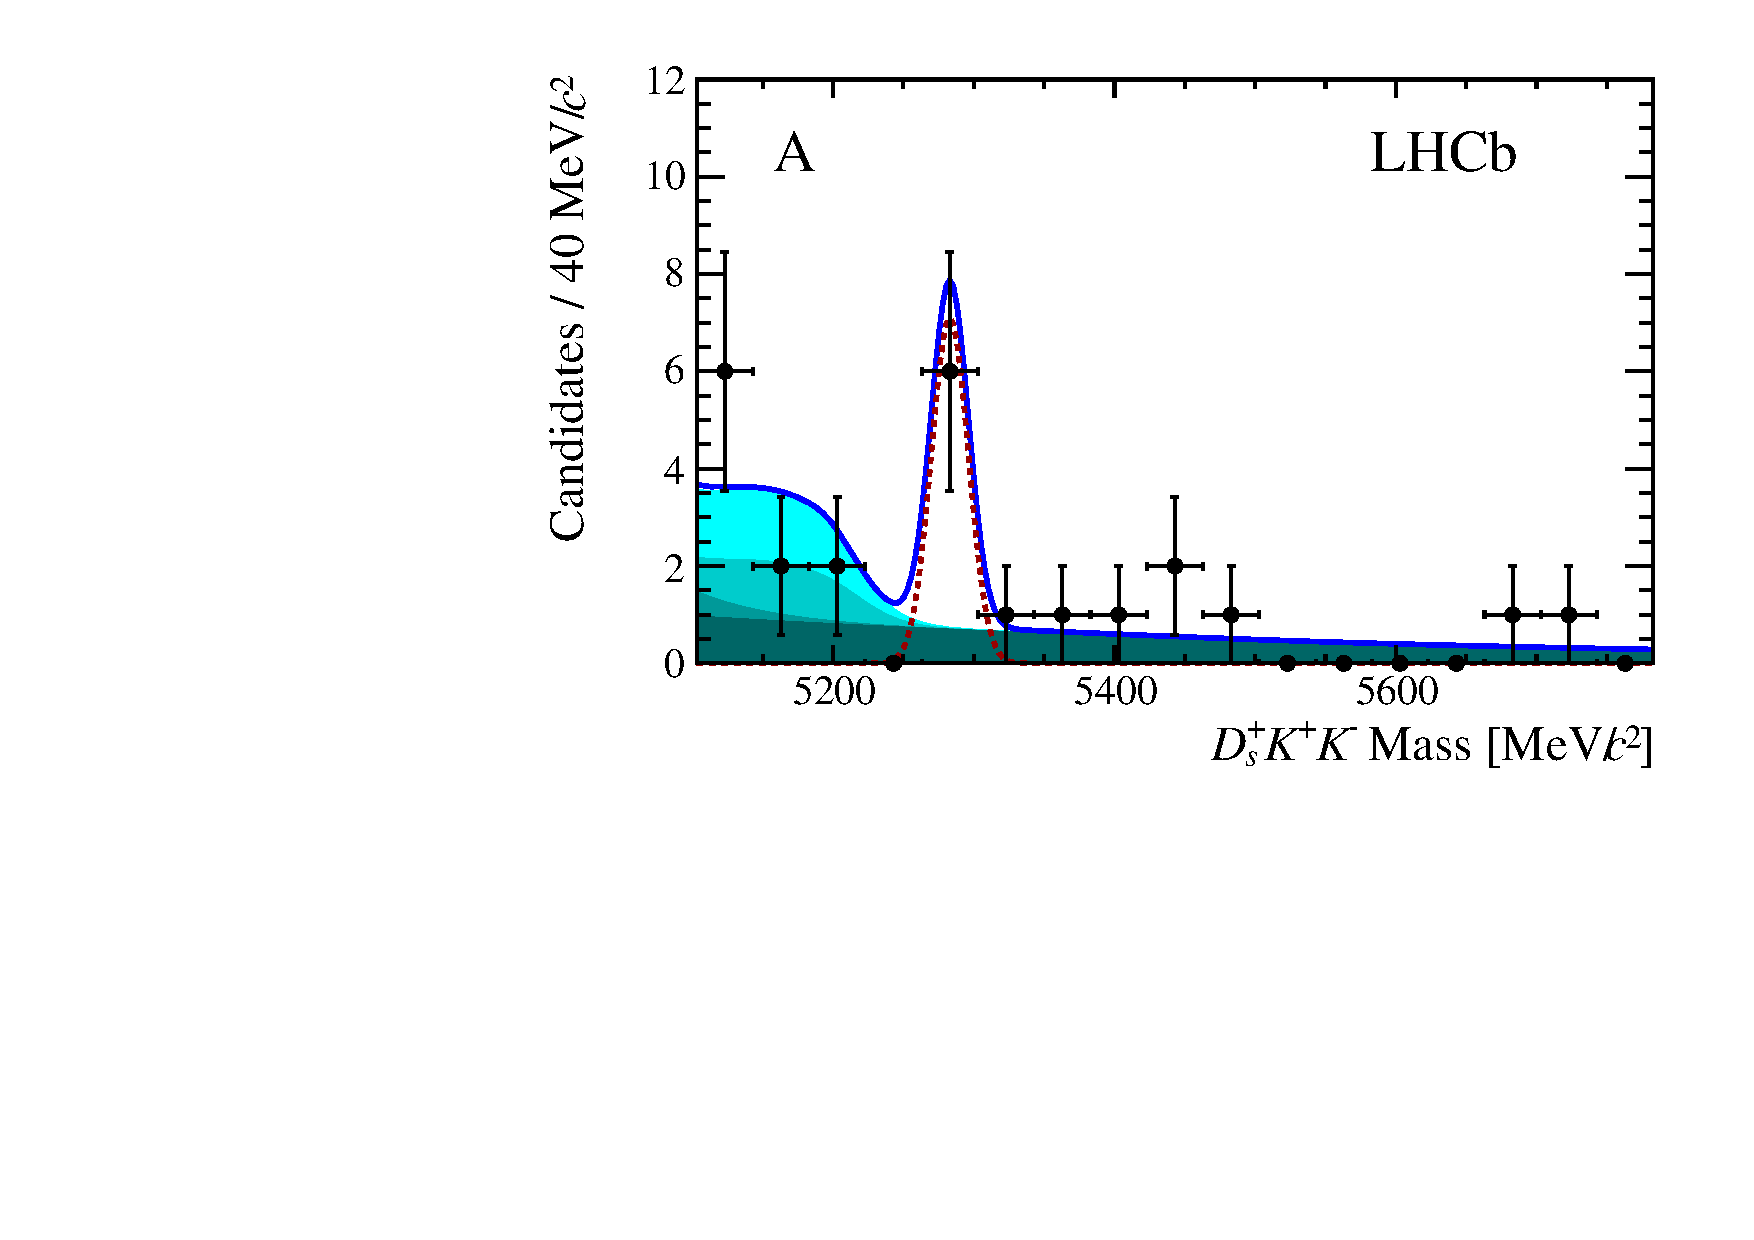
\includegraphics[width=0.48\textwidth]{B2Dsphi_regionA}
    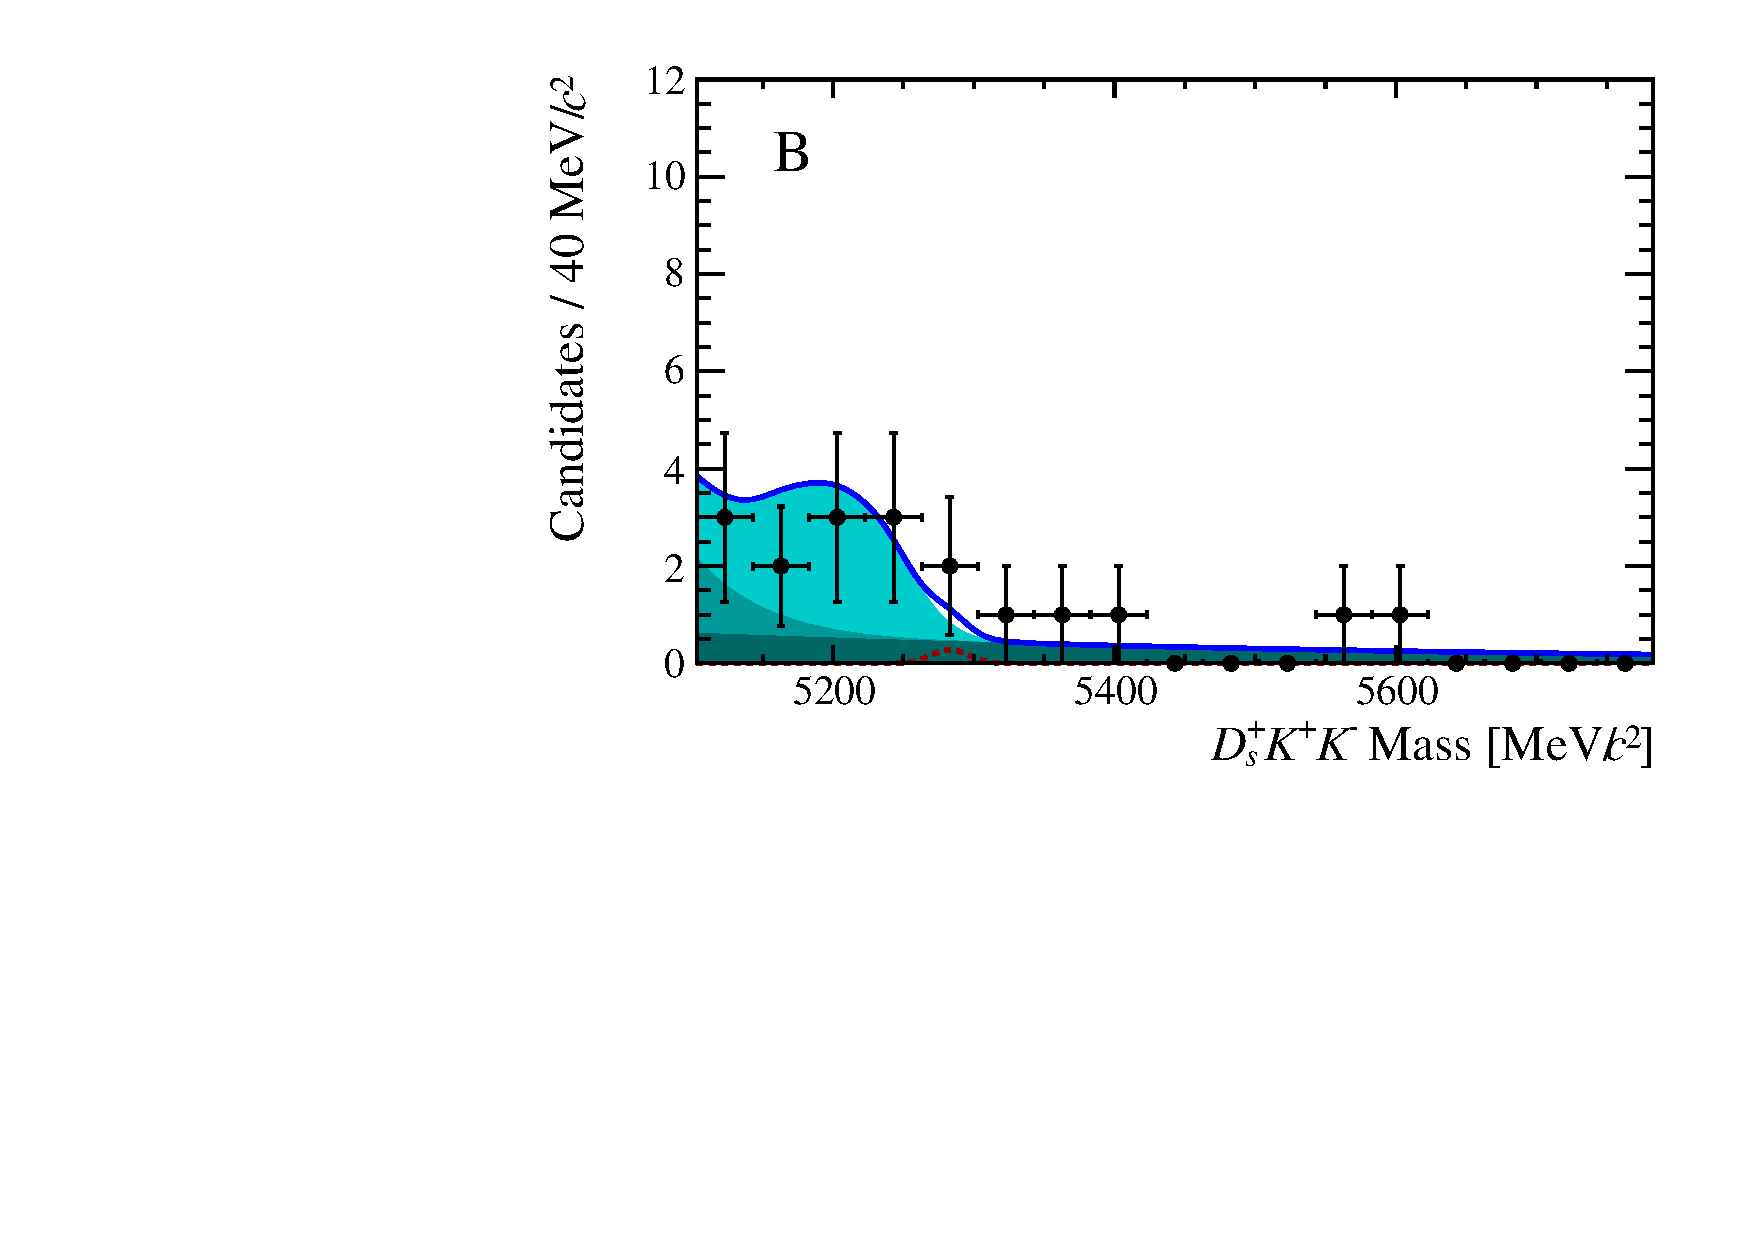
\includegraphics[width=0.48\textwidth]{B2Dsphi_regionB}\\
    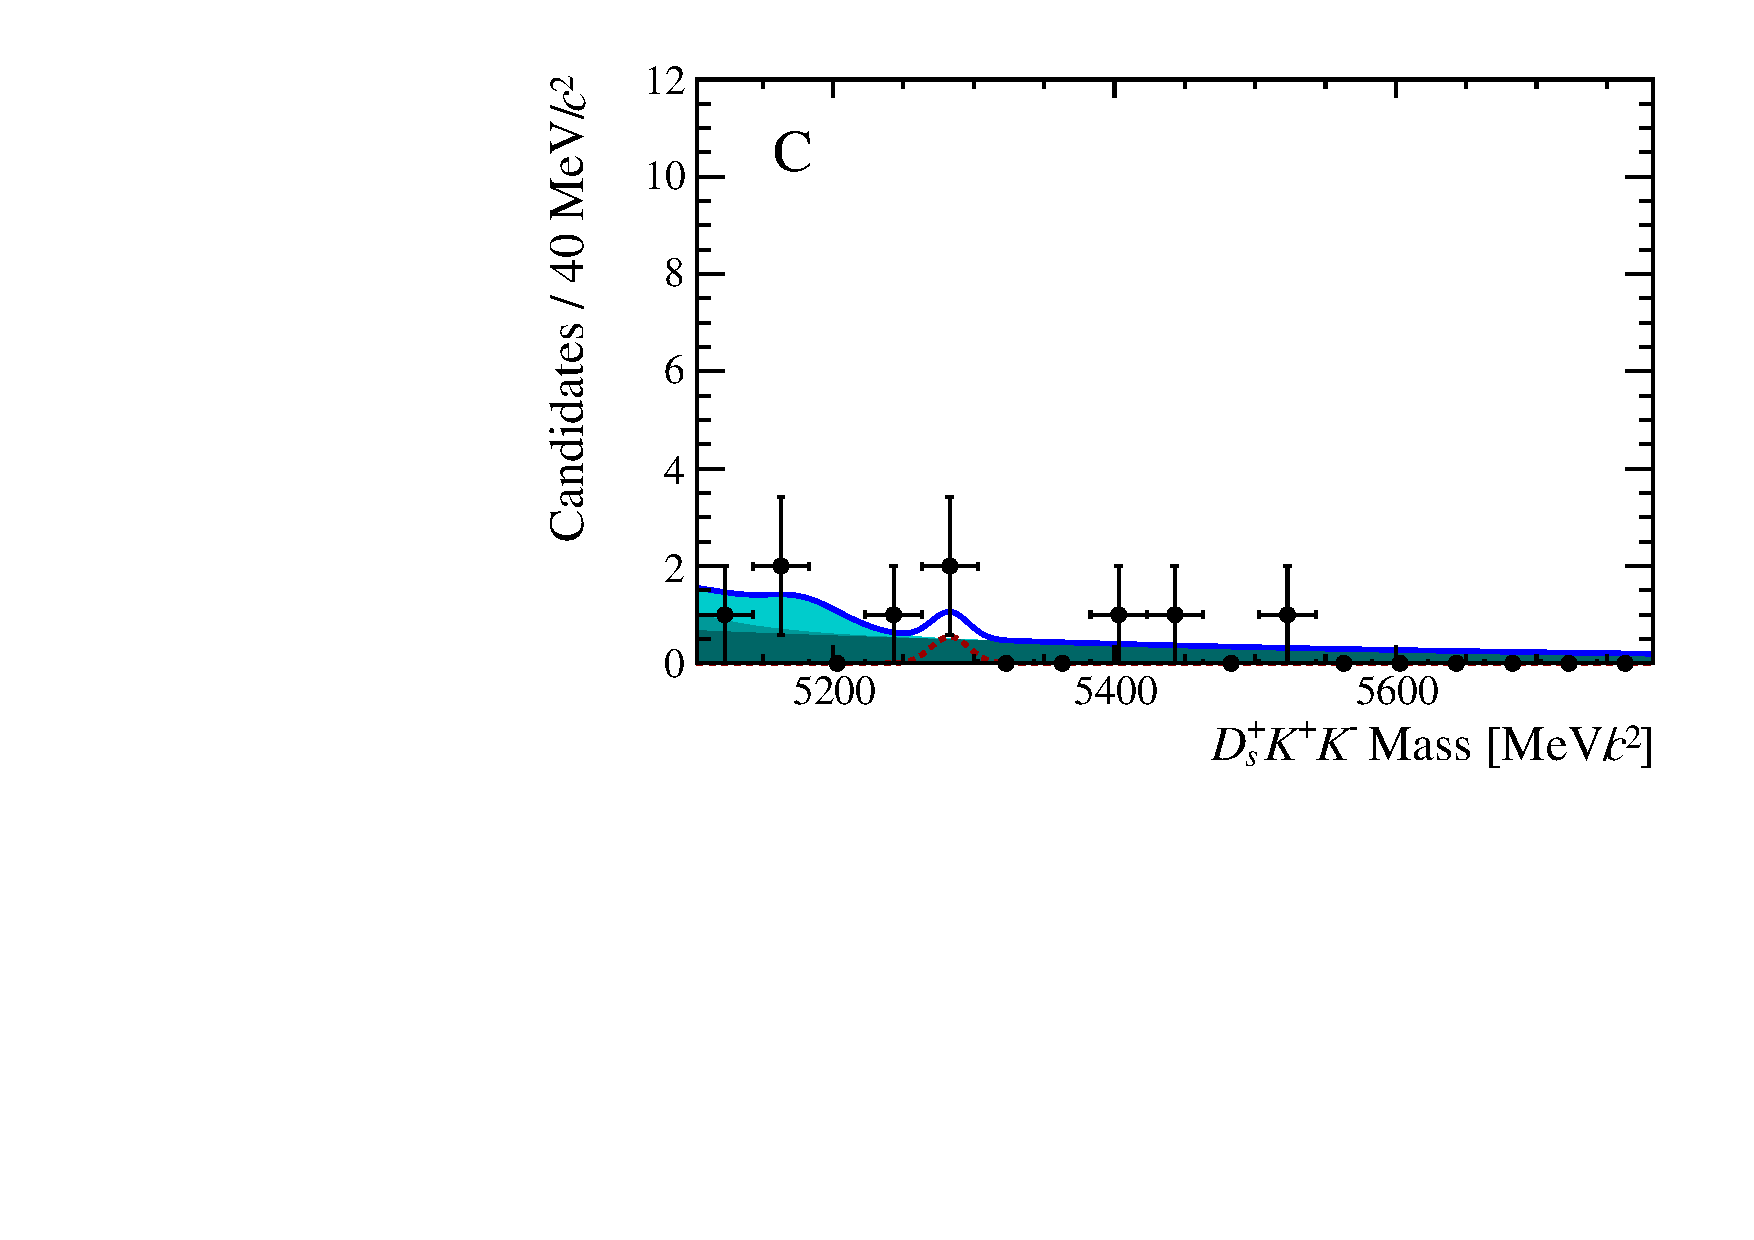
\includegraphics[width=0.48\textwidth]{B2Dsphi_regionC}
    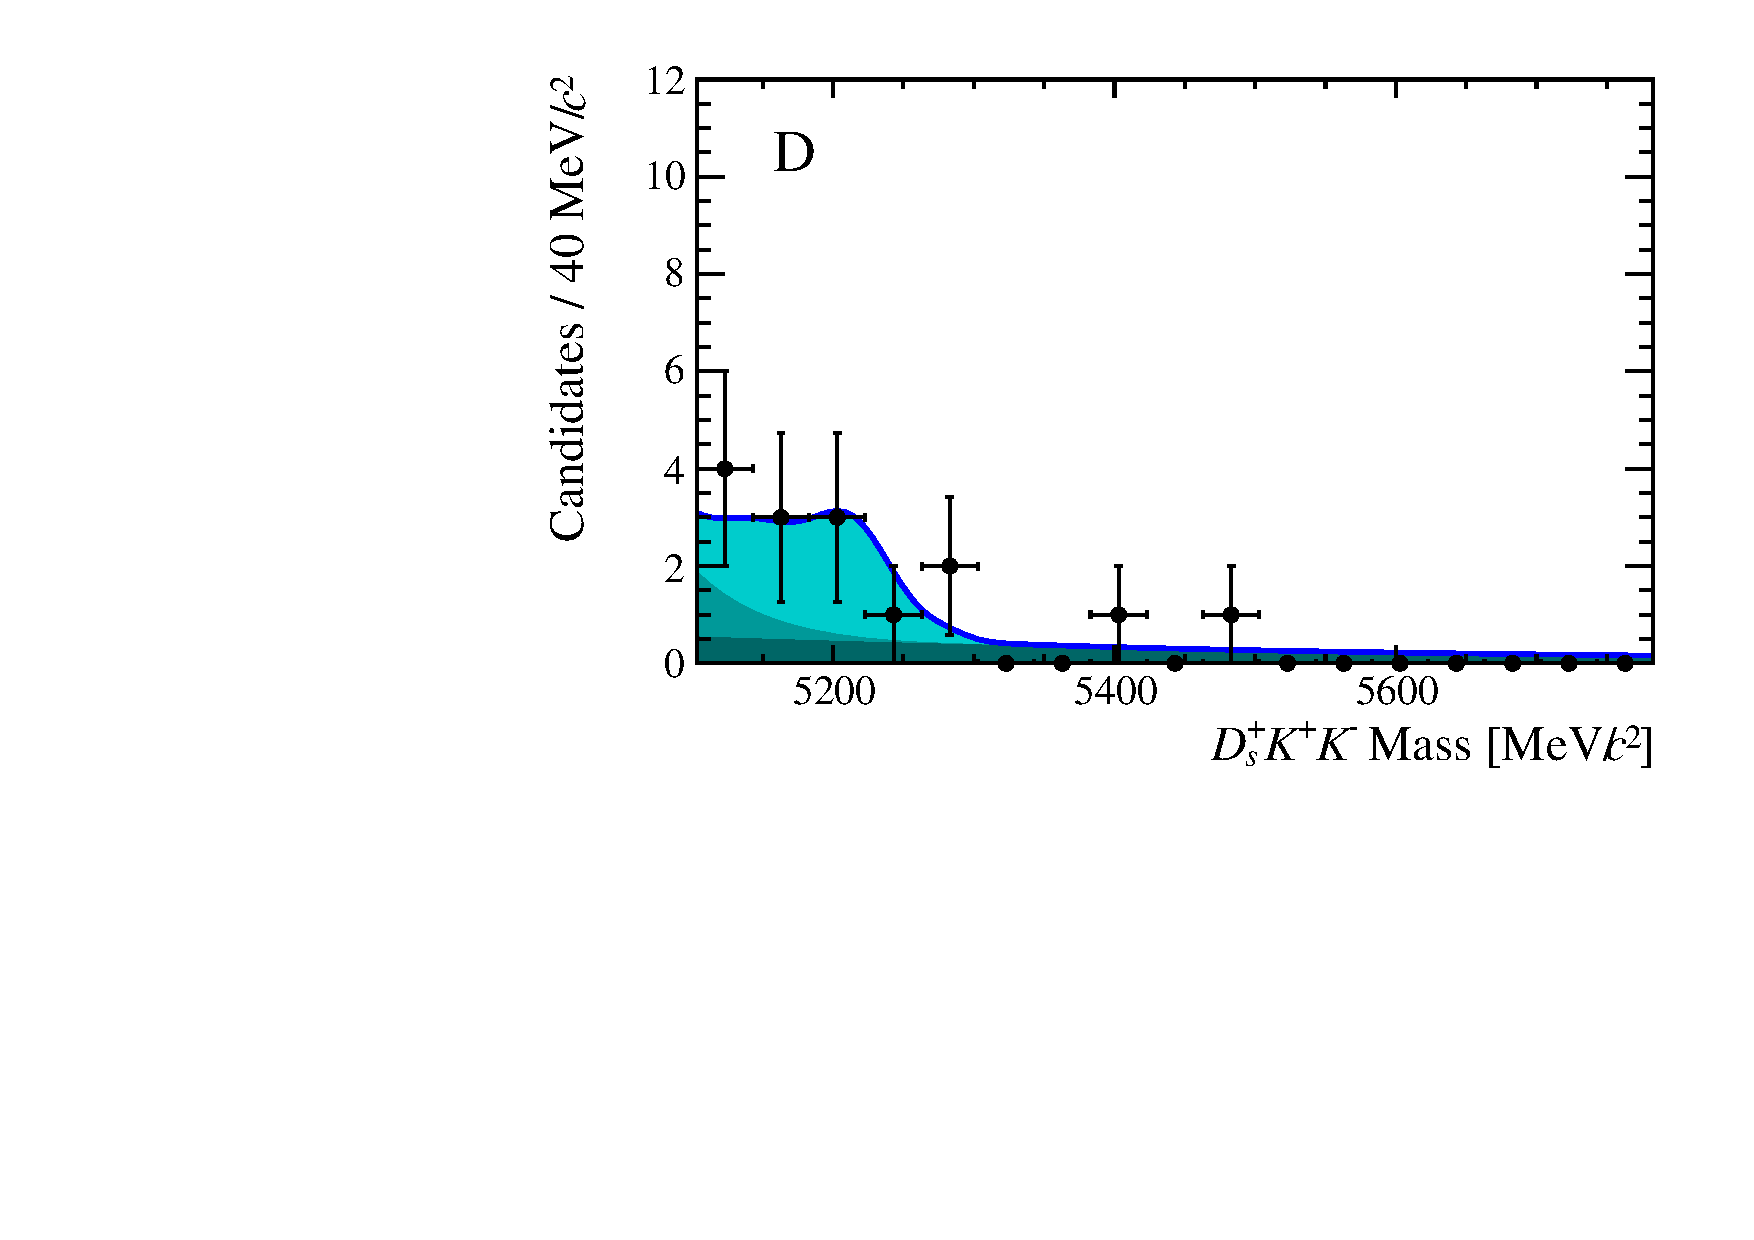
\includegraphics[width=0.48\textwidth]{B2Dsphi_regionD}
    \caption{\small
      Fits to the four analysis regions, as given in Table~\ref{tab:dsphi:hel}, in the search for
      the decay \btodsphi.
      The region \rA is contians the majority of the signal candidates, while region \rD contains
      none.
    }
    \label{fig:dsphi:fits}
  \end{center}
\end{figure}









\begin{align}
  \BF\big(\btodsphi\big) &=
  \frac{\varepsilon\big(\decay{\Bp}{\Ds\Dzb}\big)}{\varepsilon\big(\btodsphi\big)}
  \cdot
  \frac{\BF\big(\decay{\Dzb}{\Km\pip}\big)}{\BF\big(\phitokk\big)}
  \cdot
  \frac{N\big(\btodsphi\big)}{N\big(\decay{\Bp}{\Ds\Dzb}\big)} \nonumber\\
  &=\big(1.87\,^{+1.25}_{-0.73}\stat\pm0.19\syst\pm0.32\normerr\big)\e{-6}.
  \label{eq:dsphi:bf}
\end{align}



















